% Changing book to article will make the footers match on each page,
% rather than alternate every other.
%
% Note that the article class does not have chapters.
\documentclass[letterpaper,10pt,twoside,twocolumn,openany]{book}

% Use babel or polyglossia to automatically redefine macros for terms
% Armor Class, Level, etc...
% Default output is in English; captions are located in lib/dndstring-captions.sty.
% If no captions exist for a language, English will be used.
%1. To load a language with babel:
%   \usepackage[<lang>]{babel}
%2. To load a language with polyglossia:
%   \usepackage{polyglossia}
%   \setdefaultlanguage{<lang>}
\usepackage[english]{babel}
%usepackage[italian]{babel}
% For further options (multilanguage documents, hypenations, language environments...)
% please refer to babel/polyglossia's documentation.

\usepackage[utf8]{inputenc}
\usepackage{lipsum}
\usepackage{listings}
%\usepackage{tikz}

% dnd package options 
% bg-full   : Default option. Use paper background and fancy footer.
% bg-print  : Use fancy footer but not background.
% bg-none   : No paper background and plain footer.
% justified : Use full justification for text layout instead of ragged right.
\usepackage{dnd}

\lstset{%
  basicstyle=\ttfamily,
  language=[LaTeX]{TeX},
}

\title{Underdark}
\author{ocket8888}

\usepackage{eso-pic}
\newcommand\BackgroundPic{%
\put(0,0){%
\parbox[b][\paperheight]{\paperwidth}{%
\vfill
\centering
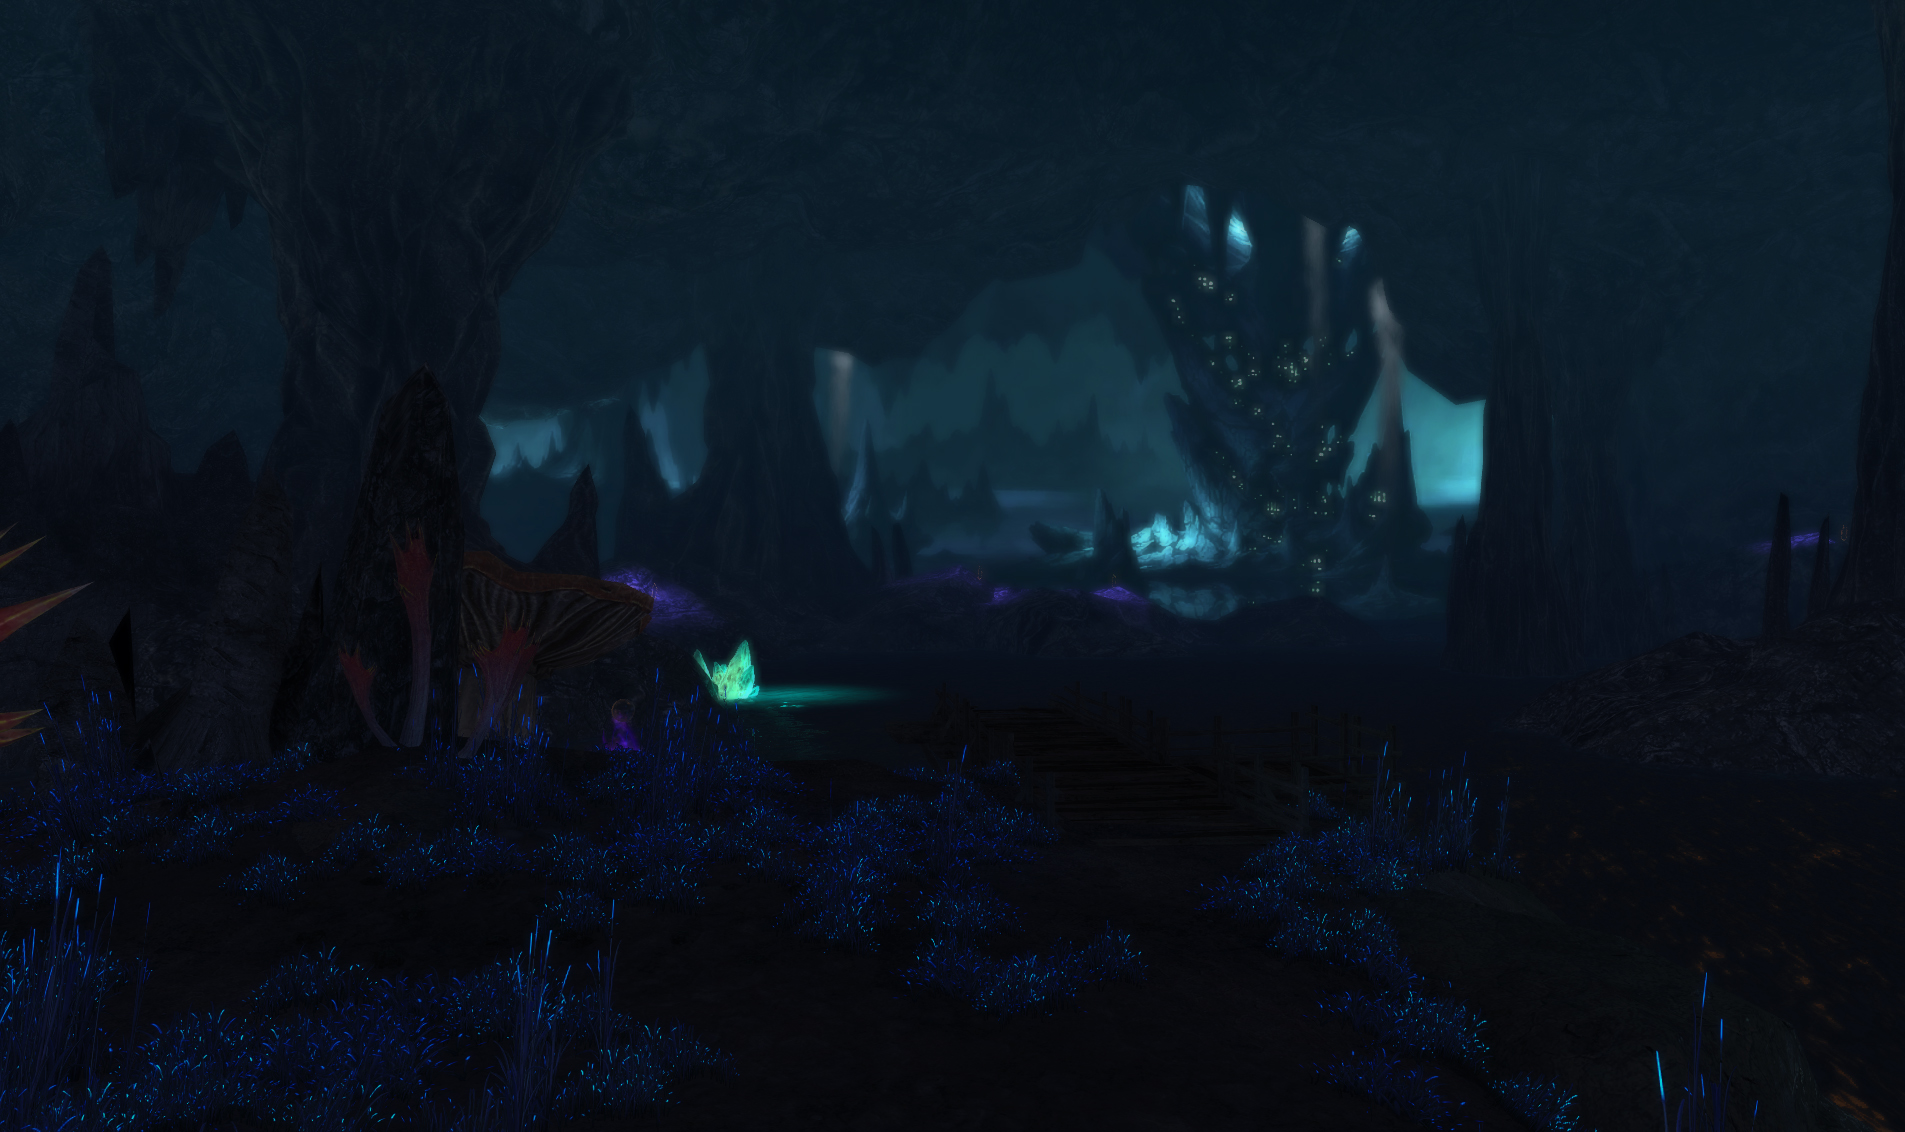
\includegraphics[width=\paperwidth,height=\paperheight]{underdark.jpg}%
\vfill
}}}

\usepackage[pdfusetitle,
			pdfsubject={Fantasy},
			pdfkeywords={Dungeons and Dragons, Roleplaying, Fantasy, Adventure},
			pdfproducer={MikTeX},
			pdfcreator={XeLaTeX}]{hyperref}

\usepackage{fontspec}
\usepackage{xunicode}
\defaultfontfeatures{Mapping=tex-text}
\setmainfont{ScalaSans}
\setsansfont{Dungeon}
\titleformat*{\chapter}{\Huge\sffamily}


\pagestyle{fancy}
\thispagestyle{plain}

% Start document
\begin{document}
\AddToShipoutPicture*{\BackgroundPic}
\begin{titlepage}
\centering

\includegraphics[width=0.5\paperwidth,keepaspectratio]{img/title.pdf}\\
{\Large \color{white} \textasciitilde{} The Captive Chronicles Pt. 1 \textasciitilde}
\end{titlepage}

\chapter*{Introduction}
Deep beneath the surface of the world lies the Underdark. a realm of endless labyrinthine tunnels and caverns where the Sun never shines. The Underdark is filled with races and creatures too numerous to count or list, and foremost among these are the dark elves- the drow. Hated and feared even by their fellow dwellers in darkness, the drow raid other settlements in the Underdark as well as the surface world, taking prisoners back with them. Rendered unconscious with drow poison, then collared and shackled, these prisoners are eventually sold as slaves or entertainment in the dark elves' subterranean cities. 

Our adventurers have all had the misfortune of falling to such a fate. Captured by the drow, they are prisoners at one of the Drow's outposts awaiting transport to the great slave city of Menzobarranzan, the city of spiders.

\chapter{1. Captive}
In the suffocating, malodorous dark of large cell in the Drow outpost's prison, a scheme was being formulated. The man doing the scheming, a tall Wood Elf in his mid 20's with short, messy, chestnut colored hair and emerald eyes, was named Dox Evenwood, and he felt that he and his companion Jhank had spent far too long in the cell already. Jhank was a hulking 7ft Lizardman, with olive-green scales and a bright orange/yellow fin protruding from the top of his head to about his shoulder blades. Both were frustrated with their situation, but Jhank was approaching furious.\\

The cell in which the prisoners found themselves was quite large, and contained numerous exotic beings. By the dim, flickering torchlight, one can just make out the rocky walls of the enclosure, one of which played host to a row of chamberpots that the prisoners were made to empty each day by flinging their contents over the side of a gaping abyss just outside the cell doors. The rush of water could be heard faintly, as a waterfall poured over the side into fathomless black.\\

With the recent arrivals, Dox felt confident an escape attempt was within their grasp. Already incarcerated upon their arrival was a host of interesting and potentially instrumental characters.\\

Most unusual among them was what appeared to be a huge mushroom that stumbled around the cell on stumpy legs. It stood approximately 3.5 feet tall, and seemed to move back and forth somewhat fretfully, avoiding other prisoners. Occasionally, it would emit a puff of reddish particulate into the air from its cap. Prisoners have noticed that standing near the mushroom-man caused them to hear voices in their head, saying things such as "...the grove remembers..." and "...must return to the others...".\\

Another of the more reclusive prisoners was a large, pensive toad-like creature that seemed content to pass its time sitting by a wall. The fish-man rocked back and forth and periodically issued gutteral noises from deep within its throat. Despite the somewhat threatening size of the fish-man and the low, growl-like noises he was making, he appeared to be quite approachable, looking at those who passed nearby with a sort of mild, calm interest.
\begin{center}
	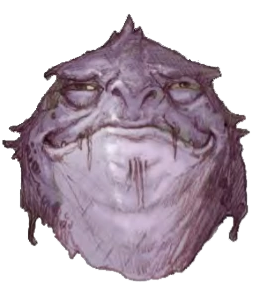
\includegraphics[width=0.45\textwidth]{img/src/fish_man.png}
\end{center}

In contrast, a large orc also co-inhabited the cell, and he appeared quite aggressive. The orc was clearly no stranger to fights, as it was heavily scarred and missing half of one tusk. The monster occasionally shot glares at Jhank, seemingly perceiving him as a threat (which Jhank responded to with casual indifference), and was never afraid to bellow at the guards, threatening all manner of colorful death and dismemberment.\\

Dox and Jhank had been languishing in a Drow prison for the past ten days. In that time, the pair and their fellow incarcerated had begun hoarding potentially useful objects that their captors had dropped or otherwise overlooked. Dox had managed to collect an crossbow bolt that had an odd smell, and Jhank concealed a rusty iron bar on his person. Shortly after their internment, the Drow Elf Danixoth had appeared, and somehow since then he had come into possession of a dull ruby and some gold pieces. One day ago, a Dwarf named Jurnthar Ironback arrived from a mining colony. Today, three new prisoners were thrown in. Adran Oakenheel the Wood Elf druid managed to fashion a makeshift 5 foot rope out of collected spider-webbing, Alchemist the Kenku gathered some gold pieces and Nithe the Tiefling managed to crack a shard of flint off of another rock while smashing rocks together out of boredom one night.\\

By comparing stories of their capture, the prisoners deduced that they had been drugged. As they were discussing this, a somewhat large tarantula hesitantly approached Jurnthar, seeming passive and as friendly as an arachnid can. Jurnthar whistled to the creature and extends a friendly hand, and it initially recoils, but is soon coaxed to a perch on the dwarf's shoulder. Adran looks about himself and sees that the ceiling 15 feet above them is engraved, though cannot make out the engravings. The door to the cell has two iron bar gateways. The cell contains a few chamberpots, which the prisoners have been made to empty several times.\\

A Drow routinely clutches the bars of the cell and nervously mumbles to himself "I am not guilty!" "I did not do it!" and he seems desperate to escape back to his former life.

A bald, purple-headed creature covered in grime is horrid to look at, but it belies an upbeat and positive nature, and a love of gambling. It is from his vast stash of gold that Alchemist and Danixoth 

A dwarf with tribal tattoos and parts of his head shaved sits against the wall. His clothes are torn in an effort to be more intimidating. He does not get along well with the orc and wishes to return to his dwarven home

Quigoth monster, the species which was observed to be used as the Drow's hired muscle. This Quigoth, however, appears to be grooming itself and standing straight in efforts to appear more civilized, if not friendly.

A thin, dwarf-like creature in tattered robes and two underdeep gnomes (which whisper between each other but refuse to communicate with others and appear to be twins)\\

Alchemist approaches the mushroom-like creature and examines it, which reveals nothing of its mysterious nature. Danixoth attempts to communicate with the creature, saying "Hey buddy, I don't mean to intrude, I know you don't like talking to us, but I was wondering - What's your name?"

"M-m-my name is Stool..." came the timid response. The creature had pressed itself back into the corner as far as it could go.

Meanwhile, Jhank approaches the Drow by the cell door and demands "What brought you here, captured by your own people?"

The Drow turns and replies "You have no place speaking to me, animal."

Dox, hearing this approaches and slaps the Drow in the face, while Jhank balls up the Drows hand in his reptilian claw and asks again "Why are you here?"

The Drow coldly states "I will not be threatened by a beast."

Not willing to actually hurt the man, the two adventurers retreat. Nithe approaches the group and attempts to calm the group down, "Alright now, we're all in here together. No sense doing the guards' work for them.". The Drow seems to notice how outnumbered he is, and quickly apologizes saying "I'm sorry, I'm just frustrated, I don't belong in here you see; I'm innocent."
"We're all in that situation, just let's all help each other, yeah? I know we don't know you, but we're just trying to help. Let's work together."
The Drow walks away saying "I'm sorry, you're right I need to calm down" and walks away, bumping into Jhank - intentionally, it seemed.

Nithe extends his hand to Jhank and Dox with the introduction "Well met, I'm Nithe" "hi im keif"

The purple man approaches Alchemist and offers a bet, "I bet you that Drow dies by morning, care to take that action?" to which Alchemist replies "How about something more interesting, I bet that if the orc and quigoth could be made to fight, the quigoth would handily win. Say, three gold pieces?" "Done"

The purple man approaches the orc and says "Hey fuckhead, that guy said you fuck goats" and points at the quigoth. The orc runs over to the quigoth and begins screaming about how it would dismember it, but the quigoth says "No sir, I did nothing of the sort, and I mean you no harm."

The adventures then hear a clamoring from outside the cell, as guards approach and bark out "No fighting!". The orc rounds on the guards and screams "Why don't you get in here and try to stop me!" to which the guards respond by drawing their crossbows and warning the orc to back off, but he doesn't listen and one bolt lodges itself in his shoulder while the other slams into his leg. The orc stumbles forward one step and falls to the ground, unconcious. The drow reload and warn Jhank, Nithe and Dox and demand that they retreat from their position by the door, now backed with Quigoth muscle. One drow and two quigoth enter the cell, and drag the orc out, and then away into the hallway.

Alchemist remarked to the purple man "I guess our bet's off". The Quigoth approaches the purple man and protests "I never said that, why did you say I said that?!?" but the purple man just laughs and walks away, flipping a coin in his hand.

Jurnthar approaches the thin, dwarf-like man and asks "How's it going, brother?", mistaking him for a dwarf. "A lot better now that that filthy orc isn't in here anymore"
"I see you got a lot of tribal tatoos, friend, what's up with that? My name's Jurnthar, by the way."
"I am Wedgrar Greckan Warriors, my tribe were hunting stinkin' orcs like that when I was captured."
"What manner of fighter are you?"
"I cleave"
"Sounds like we'd make a good team; I shoot. These others appear"
"Whatever gets me to Grontilgrim"
"I hear that. When we get there I'll buy you a flagon of mead"
"Aye, and one for you too"
"It's good to meet a fellow dwarf in here"

Dox approaches the Quigoth and asks "Hail. How is it that you are in here"

Ah yes, my appearance. You see, I'm actually an elf. My name's Darandil a prince from the Nelandril forest.
That sucks.
Quite.

Danixoth approaches the other drow and says "I can see by your clothing that you are not low-born, how came you here?"
"Another Drow, thank god. Are you from Menzobaranzan?"
"No, but I am familiar with the area."
"I had to run, and these guards - knowing what I am accused of - want to sacrifice me to Lolth. But I am innocent"
"I too, am fleeing false persecution. Do you have any plan to escape? I see you at the bars mumbling sometimes, is that part of a plan?"
"It's the only thing I can think to do. I'm a drow, surely I deserve a trial?"
"Don't we all"

Alchemist approaches the fish man, and mimicks his low growling noises. The creature's eyes snap open with an agility that was unexpected for a beast of his size, startling Alchemist a bit, but he quickly recovers and the two gurgle at each other. Alchemist turns around and asks Jhank, "Hey, you look weird, he looks weird, you guys know each other?" Jhank merely scoffs and turns away, but the fish man spoke "Do you wish to be awakened?"
"In what way?"
"Violence is a circle, I represent peace"
"Okay, so how do I 'awaken'?"
"Join me on my path of peace, we can better this world"
"Actually, I'm good"
The fish man appears unfazed.

Adran examines the etchings on the ceiling, and notices that they glow a bit. Not enough to cast light in the cell, but just enough to be noticeable. Danixoth notices that they have no Lolth religious significance, and Adran senses some amount of magic emnating from the runes. 

Nithe meditates to attempt to commune with Bahamut.

Jurnthar approaches Adran and asks "What's your name, tree boy?" "Adran" "I'm Jurnthar. You're a shapeshifter, right?" "I am a druid, but I cannot yet shapeshift." "oh, I thought maybe you could turn into a spider" "I cannot" "Well if you ever need to, feel free to study my spider" "Actually I was hoping to get a sample of silk to compare to my rope" Jurnthar politely asks "Can we have some silk?" the tarantula blinks and poops some silk into Jurnthar's hand, which he then gives to Adran, who does nothing with it, which was weird. Jhank approaches the underdeep gnomes and asks "What's your deal?" from close up he could tell that one was male and the other female. The mail recoils and the female snaps "we don't talk to outsiders!", and Jhank retreats.

Dox pulls Jhank aside and lays out his plan "There's no way an orc that size was taken out by two non-lethal crossbow shots" and pulls out his strange-smelling bolt "I believe these to be coated" let's get 'em otay alchemist gets shut down yadda yadda

Danixoth approaches Nithe, who had finished meditating and asks "Did you catch that? Do you think we could help?" "I suggest we not let them get killed, and try not to draw attention" "let's get that shroom, dawg" "don't group up"

The other Drow approaches Alchemist and asks "Would you kindly remove yourself from my Stool's presence?" Alchemist wordlessly retreats back to the fish man, and the Drow and Stool appear to have a telepathic conversation.

Danixoth approaches and inquires "I forgot to get your name, sir" "My name is Carith Kzekarit" "I go by Danixoth. I see you know this mushroom. How far away can a mind be touched by it?" Carith explains that this creature is a Michonid that lost his name. He named it "Stool" because he used it as a seat. The spores, when clinging to a person, provided a telepathic communication channel within roughly 15 feet. Danixoth asks if Stool could be convinced to sit in a more central position. Carith glares at the mushroom, which moves to the center of the room and plops down onto the ground "Thank you" "Drow don't thank."

>spreads the plan to Jurnthar

>Jurnthar fills in his pal Wedgrar. The guard Drow clangs his sword against the cage and shouts out "Quiet down in there."

>Jhank fills in Darandil, who finds him fascinating

>Jhank signals that he's ready 

>spores get set up

>Jhank punches Darandil

>Diirka Deero

\section{Awake}


\end{document}